\documentclass[aspectratio=169]{beamer}

\usepackage{basileabeam}
\usepackage[most]{tcolorbox}


\addbibresource{presentation.bib}
% Notes:
%\pgfpagesuselayout{2 on 1}[a4paper,border shrink=5mm]
%\setbeamertemplate{note page}[plain]
%\setbeameroption{show notes on second screen=bottom}

\title              {Application of Graph Learning to inverse problems}

\author     		{Cédric Mendelin}
\email				{cedric.mendelin@stud.unibas.ch}
\institute          {Department of Mathematics and Computer Science, University of Basel}

\date               {Date}

\ulogo        		{Template/header}
\ulistelement    	{Template/listelement}

\graphicspath{{Figures/}}

% Options:
%\totalNoSlidesDisabled % To turn off the total number of slides in the footer. Comment this if you want the total number of slides in the footer

%\headerSectionsDisabled % Comment this if you want a fancy header containing your sections.


\begin{document}

\begin{frame}[t,plain]
    \titlepage
\end{frame}

\begin{frame}[t]{Outline}
    \tableofcontents
\end{frame}

%% Presentation content

\section{Imaging methods}	% You can also have slides prior to the first section or work entirely without sections.

\begin{frame}[c]{Cryo-EM}
    \begin{figure}
        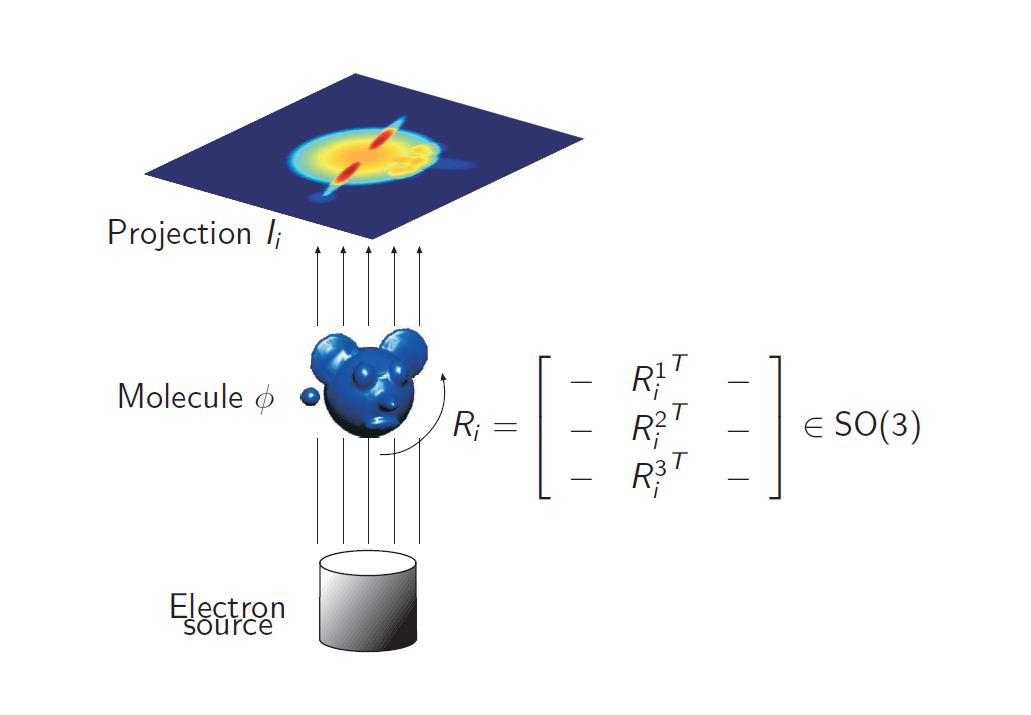
\includegraphics[width=0.4\textwidth]{cryo-EM-overview.png}
        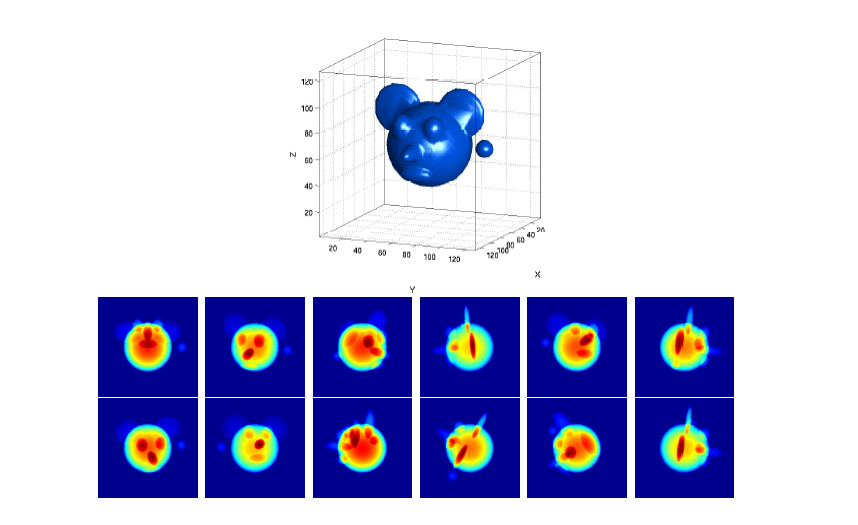
\includegraphics[width=0.4\textwidth]{micky-mouse.png}
        \caption{Cryo-EM overview \cite[Figure 1 and Figure 2]{cryoEmMath2}}
    \end{figure}

\end{frame}

\begin{frame}[c]{Cryo-EM challenges}
    \begin{itemize}
        \item High-noise level 
        \item Unknown rotation during freezing
        \item (Structural variety of observations)
    \end{itemize}

    
    \begin{tcolorbox}[colback=red!5!white,colframe=red!75!black]
        The main domain of interest is the high-noise domain (cryo-EM).
    \end{tcolorbox}

\end{frame}

%\begin{frame}
%    \begin{definition}[Cryo-EM observation]
%        $$ y_i[j,k] = \Pi_z (\; Rot(\;x; \theta_i))_{j,k} + \eta_i[j,k], \text{ with } 1 \leq i \leq N \text{ and } 1 \leq j,k \leq M,$$
%    \end{definition}
%    \begin{itemize}
%        \item $y_i[] \in \tilde{\Omega}, x \in L^2(\Omega)$ with $\Omega \subset \mathbb{R}^3 $ and $\tilde{\Omega} \subset \mathbb{R}^2 $
%        \item $M$ observation dimension
%        \item $\Pi_z : L^2(\Omega) \to L^2(\tilde{\Omega})$ projection operator
%        \item $Rot : L^2(\Omega) \to L^2(\Omega),$ is rotation operator
%        \item $Rot(x, \theta_i) = \left((x_1,x_2,x_3) \mapsto x( x_1R^1_{\theta_i}, x_2R^2_{\theta_i}, x_3R^3_{\theta_i})\right)$
%        \begin{itemize}
%            \item $\theta_i = [\theta_i^{(1)}, \theta_i^{(2)}, \theta_i^{(3)} ] $, with $\theta_i^{(1)}, \theta_i^{(2)}, \theta_i^{(3)} \in \mathbb{R}$
%            \item $R_{\theta_i} =  [R^1_{\theta_i}, R^2_{\theta_i}, R^3_{\theta_i}] \in SO(3)$ is the 3D rotation matrix 
%        \end{itemize}
%    \end{itemize}
%\end{frame}


\begin{frame}[c]{Computed Tomography}
    \begin{columns}[c]
        \column{.45\textwidth}
                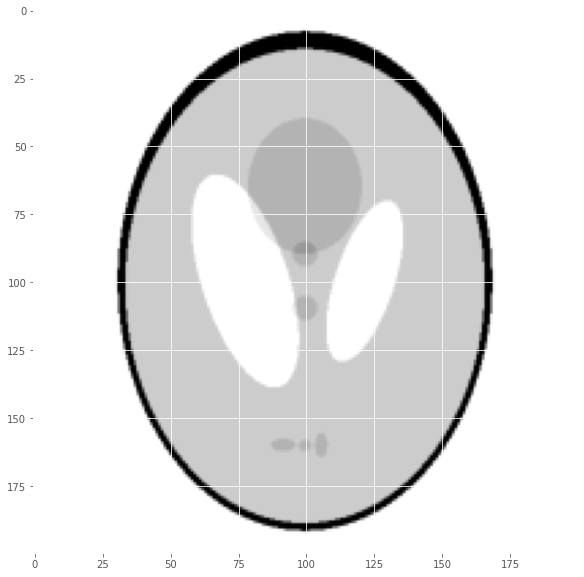
\includegraphics[width=0.4\textwidth]{phantom.png}
                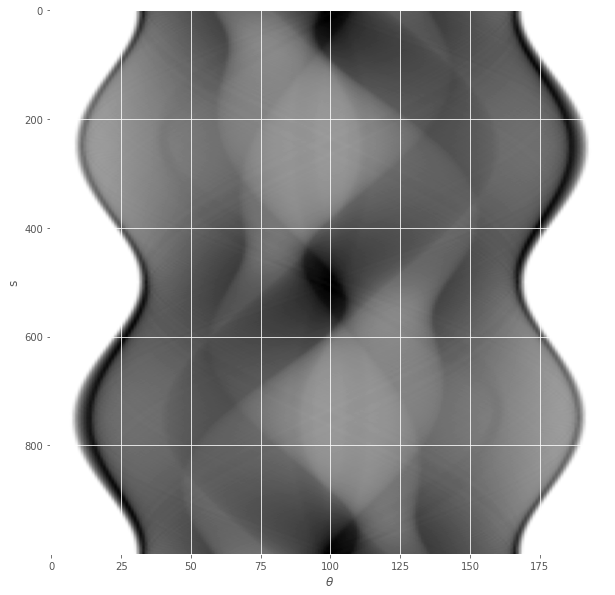
\includegraphics[width=0.4\textwidth]{phantom_sinogram.png}
                
        \column{.55\textwidth}
            \begin{itemize}
                \item Related to cryo-EM
                \item Can be seen as simpler version in 2D
                \item Good to start with
            \end{itemize}
    \end{columns}

\end{frame}

% \begin{frame}
%     \begin{definition}[CT observation]
%         $$ y_i[j] = R(x, \theta_i, s_j) + \eta_i[j] , \text{ with } 1 \leq i \leq N \text{ and } 1 \leq j \leq M,$$
%     \end{definition}
% 
%     \begin{itemize}
%         \item 
%     \end{itemize}
%     
% \end{frame}


\section{Graph Denoising}

\begin{frame}{Graph construction}
    Let $\Omega$ be a dataset $\Omega \subset \mathbb{R}^M$, a graph can be constructed like:
    \begin{itemize}
        \item $V$: each node associated with $x \in \Omega$
        \item $E$: Calculate adjacency matrix with similarity measure $d$ and some threshold $\tau$
     \end{itemize}

     \begin{definition}[Adjacency Matrix]
        \begin{equation}
            \label{eq:graphConstruction}
            A_{ij} =    
            \begin{cases}
                1  & \text{if } d(x_i, x_j) < \tau\\
                0, & \text{otherwise}
            \end{cases}
        \end{equation}
    \end{definition}
\end{frame}

\begin{frame}{Graph construction}
    Let $\Omega$ be a dataset $\Omega \subset \mathbb{R}^M$, but only observation 
    of $y = x + \eta$ (with $\eta$ drawn from $\mathcal{N} \sim (0, \sigma^2)$), 
    a graph can be constructed like:
    \begin{itemize}
        \item $V$: each node associated with $y \in \Omega$
        \item $E$: Calculate adjacency matrix with similarity measure $d$ and some threshold $\tau$
     \end{itemize}
     \begin{definition}[Noisy Adjacency Matrix]
        \begin{equation}
            \label{eq:graphConstructionNoise}
            A_{0_{ij}} =    
            \begin{cases}
                1  & \text{if } d(y_i, y_j) < \tau\\
                0, & \text{otherwise}
            \end{cases}
        \end{equation}    
     \end{definition}
\end{frame}

\begin{frame}[c]{Noisy graph}

    \begin{theorem}
        For every noisy graph $G_0 = \langle V, E_0 \rangle$, 
        there exists a noiseless graph $G = \langle V, E \rangle$.
        Both graphs consists of the same set of vertices $V$ but different edges.
        $E_0$  is defined as follows:
        $$E_0 = E \setminus  E^{-}_0 \cup  E^{+}_0,$$
        where $E^{-}_0 \subseteq E$ and $E^{+}_0 \subseteq U$ with $U$ the set of all possible edges and $E^{+}_0 \cap E = \emptyset$
    \end{theorem}

\end{frame}

\begin{frame}[c]{Graph Denoising}
    \textit{Graph denoising} is the task, to estimate a denoised graph $\tilde{G}$  
    from a given noisy graph $G_O$, with underlying original graph $G$:

    \begin{definition}[Graph Denoising]
        $$GD: G_0 \mapsto \tilde{G} \approx G,$$
    \end{definition}
    where $G_0$, $\tilde{G}$, $G$ denotes noisy, estimated denoised and original graph respectively.
    
    \begin{definition}[Graph Denoising]
        $$GD: A_0 \mapsto \tilde{A} \approx A,$$
    \end{definition}
    where $A_0$, $\tilde{A}$, $A$ denotes adjacency matrix from $G_0$, $\tilde{G}$ and $G$ respectively.

\end{frame}

\section{Conclusion}


\begin{frame}[c]{Manifolds}
    We know structure of manifolds for noiseless data:
    \begin{itemize}
        \item Computed Tomography $\to$ circle
        \item Cryo-Em $\to$ sphere
    \end{itemize}

    If data is noisy, manifold will "drift" away from noiseless manifold:
    \begin{figure}
        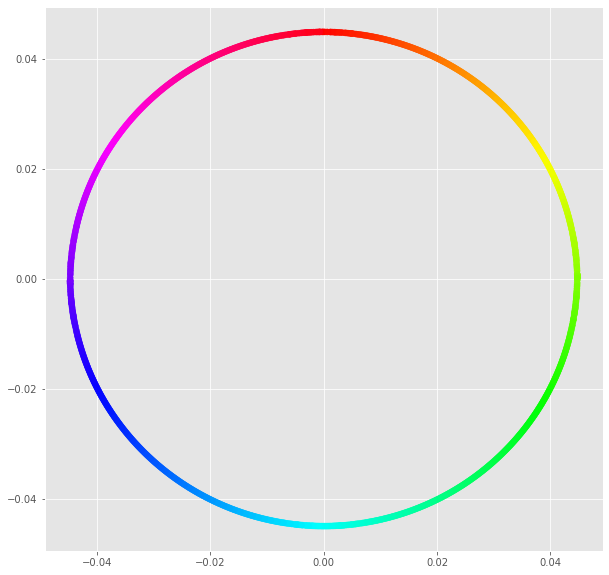
\includegraphics[width=0.25\textwidth]{phantom_second_third_evec}
        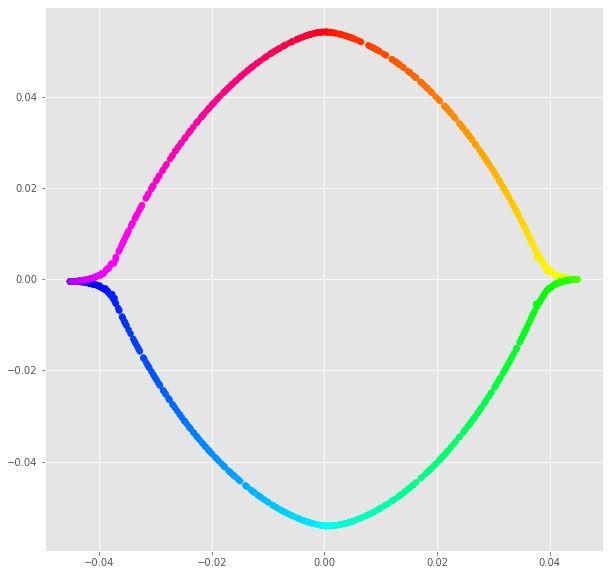
\includegraphics[width=0.25\textwidth]{phantom_second_third_evec_noisy}
        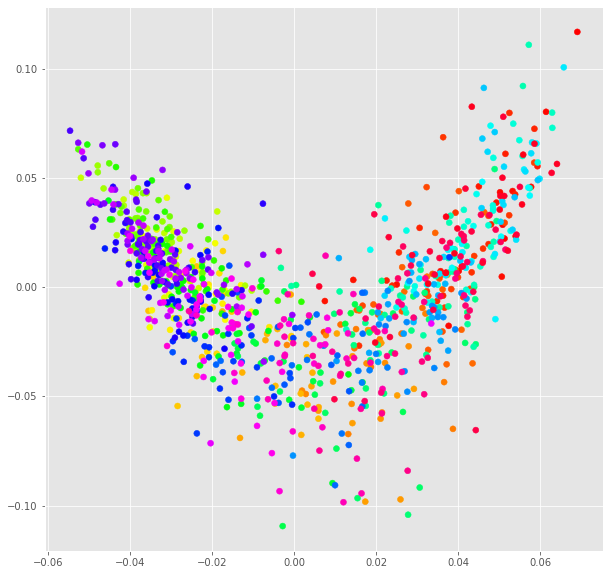
\includegraphics[width=0.25\textwidth]{phantom_second_third_evec_noisy_high}
        \caption{Manifolds for phantom without noise, and different noise levels.}
    \end{figure}
\end{frame}


\begin{frame}{Project Conclusion}
    \begin{itemize}
        \item Introduce Graph Denoising method
        \item Focus on high-noise domain (cryo-EM)
        \item Exploit known manifold in 2D and 3D
        \item Further study Graph Laplacian and connection with
            \begin{itemize}
                \item Tomography domain
                \item GNNs and Machine Learning in general
            \end{itemize}
        \item Evaluate on toy dataset in 2D and 3D
        \item Nice to have: evaluate on cryo-EM / CT dataset
    \end{itemize}
\end{frame}

\begin{frame}{Project schedule}
    \begin{figure}
        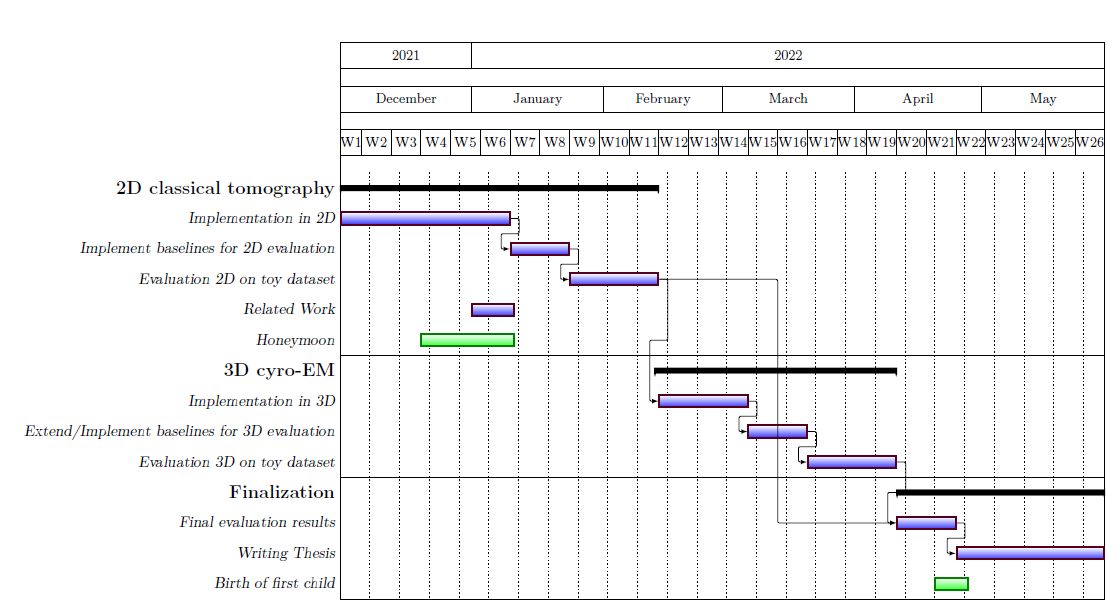
\includegraphics[width=0.8\textwidth]{gantt_chart}
    \end{figure}
\end{frame}

\begin{frame}[t,plain]
\lastpage{{\usebeamerfont{title} Questions?}\\[5ex]}
\end{frame}

\backupbegin

\begin{frame}{References}
    \printbibliography
\end{frame}

\backupend

\end{document}

